\documentclass[letterpaper]{article}

% --- Packages
\usepackage[utf8]{inputenc}
\usepackage[T1]{fontenc}
\usepackage[margin=0.25cm]{geometry}
\usepackage{enumitem}
\usepackage{pdfpages}
\usepackage{multicol}
\usepackage{amsmath}
\usepackage{amssymb}
\usepackage[skip=1pt plus1pt, indent=0pt]{parskip}
\usepackage{enumitem}
\usepackage{graphicx}

% --- Data
\title{Magnetostatic}
\author{Enrique Calderon}
\date{May 2024}

% --- Graphics path
\graphicspath{ {./img/} }

% --- Custom commands
\makeatletter
\let\thetitle\@title
\let\theauthor\@author
\makeatother
\newcommand{\compconj}[1]{%
    \overline{#1}%
}
\newcommand{\divline}{\noindent\makebox[\linewidth]{\rule{\textwidth}{0.4pt}}}
\newcommand{\taninv}{\tan^{-1}}
 
% Example of image adding
%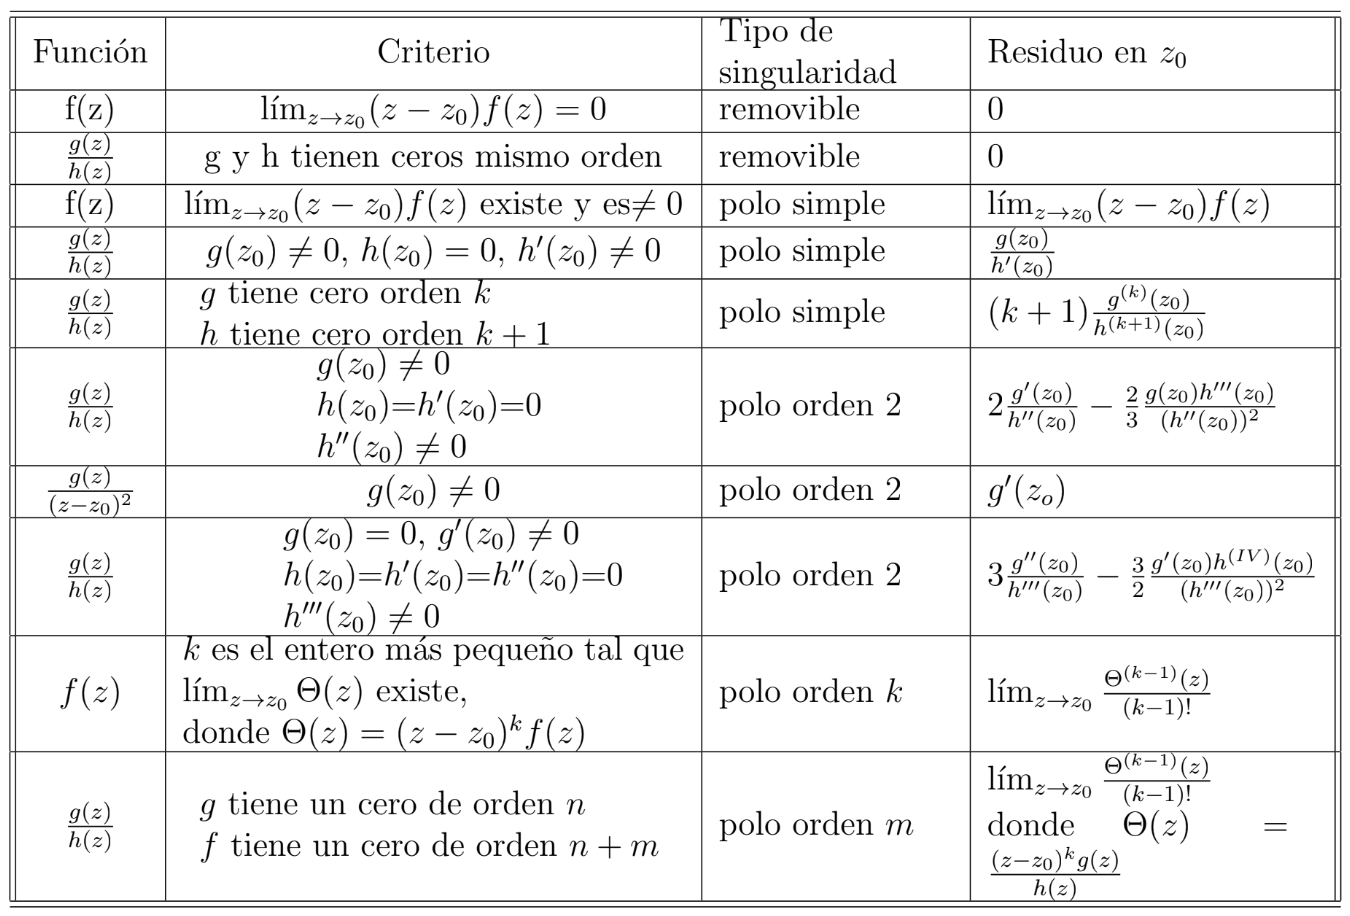
\includegraphics[width=0.8\textwidth]{ResidueTable}

% Remember to add divline between sections

\begin{document}
    \maketitle
    \divline
    
    \begin{multicols}{2}
        \section{Magnetic force with charges on movement}

        \[F_m = q v B \sin{\theta} [N]\]
        \[\overline{F_m} = q \overline{v} \times \overline{B} [N]\]
        \[ \overline{F_m} = q 
        \begin{vmatrix}
            \hat{i} & \hat{j} & \hat{k} \\
            v_x & v_y & v_z \\
            B_x & B_y & B_z
        \end{vmatrix}
        \]
    \end{multicols}
    \divline

    \begin{multicols}{2}
        \section{Magnetic field}

        \[B = \frac{F_m}{qv\sin{\theta}}\]

        \[{[B]}_u = [T] = \left[ \frac{N}{C \cdot \frac{m}{s}} \right] = \left[ \frac{N}{A \cdot m} \right] = {10}^4 [G] \]

        \begin{enumerate}
            \item It starts at north and goes to south pole.
            \item The lines do not cut.
            \item The tangent indicates the direction of the magnetic field vector.
            \item The number of lines is proportional to the magnetic field value.
            \item The magnetic field intensifies in the poles.
            \item Where they converge the field is more intense.
            \item Points indicate lines going out, x indicate lines going in.
        \end{enumerate}
    \end{multicols}
    \divline

    \begin{multicols}{2}
        \section{Lorentz, electromagnetic force}

        \[\overline{F_E} = q \overline{E} [N]\]

        \[\overline{F_m} = q \overline{v} \times \overline{B} [N]\]

        \[\overline{F_{Em}} = q [\overline{E} + \overline{v} \times \overline{B}] [N]\]
        
    \end{multicols}
    \divline

    \begin{multicols}{3}
        \section{Biot-Savart law }

        \[d \overline{B_P} = \frac{\mu_0 I}{4 \pi} \frac{d \overline{l} \times \hat{r}}{r^2} [T]\]
        
        \[d B_P = \frac{\mu_0 I}{4 \pi} \frac{d \overline{l} \sin{\alpha}}{r^2} [T]\]
        
        \[\mu_0 = 4 \pi \times 10^{-7} \left[ \frac{T \cdot m}{A} \right] \text{ ó } \left[ \frac{wb}{A \cdot m} \right]\]

        For a straight conductor segment:
        
        \[B_P = \frac{\mu_0 I}{4 \pi a} (\cos{\theta_2} - \cos{\theta_1} ) [T]\]

        For a very large segment \((l > 10 a)\)

        \[B_P = \frac{\mu_0 I}{2 \pi a} [A]\]

        \[\overline{B_P} = \frac{\mu_0 I}{2 \pi a} \hat{u} [A]\]

        For a circular spiral conductor:

        \[B_P = \frac{\mu_0 I}{2 r} [T]\]

        \[\overline{B_P} = \frac{\mu_0 I}{2 r} \hat{u} [T]\]

        For a Spiral-shaped coil conductor, with N spins :

        \[B_P = \frac{\mu_0 N I}{2 r} [T]\]
        
        \[\overline{B_P} = \frac{\mu_0 N I}{2 r} \hat{u} [T]\]

        For a square shaped coil conductor, with N spins:

        \[\overline{B_P} = \frac{2 \sqrt{2} \mu_0 N I}{\pi l} \hat{u} [T]\]

        For a circular spiral conductor outside of the plane:

        \[\overline{B_P} = \frac{\mu_0 I a^2}{2{(a^2 + b^2)}^{3/2}} \hat{u} [T]\]
        
        For a square spiral conductor outside of the plane:
        
        \[\overline{B_P} = \frac{\mu_0 I l^2}{2 \pi a^2 b } \hat{u} [T]\]
    \end{multicols}
    \divline
    
    \begin{multicols}{2}
        \section{Ampere law}

        Mathematically describes the relationship of the magnetic field to The cause that produces it: the electric current.

        \[c = \oint \overline{B} \cdot d \overline{l} = \mu_0 I_{\text{enc}}\]

        Electric field from a straight conductor:

        \[B = \frac{\mu_0 I}{2 \pi a} [T]\]

        \[\overline{B} = \frac{\mu_0 I}{2 \pi a} \hat{u} [T]\]

        Electric field from a solenoid:

        In the center:

        \[B_C = \frac{\mu_0 N I}{l} [T]\]

        In the edge:

        \[B_{\text{ext}} = \frac{B_C}{2} [T]\]

        Electric field from a toroid:

        \[B = \frac{\mu_0 N I}{2 \pi r} [T]\]
        
        \[\overline{B} = \frac{\mu_0 N I}{2 \pi r} \hat{u} [T]\]
        
    \end{multicols}
    \divline
    
    \begin{multicols}{2}
        \section{Magnetic flow}

        \[\emptyset_m = \overline{B} \cdot \overline{A} [wb]\]
        
        \[\emptyset_m = \overline{B} \cdot \hat{n} A [wb]\]

        \[1 [wb] = 1 [T \cdot m^2]\]

        By straight and large conductor:

        \[\emptyset_m = \frac{\mu_0 I h}{2 \pi} \ln{\left(\frac{r_2}{r_1}\right) [wb]}\]

        \begin{itemize}
            \item \(r_1\) : Minimum distance between the conductor and the nearest side of the surface.
            \item \(r_2\) : Minimum distance between the conductor and the farthest side of the surface.
        \end{itemize}

        By a solenoid:

        Inside:

        \[\emptyset_m = \frac{\mu_0 N I A}{l} [wb] = B_C A [wb]\]

        In the edge:

        \[\emptyset_m = \frac{\mu_0 N I A}{2 l} [wb] = B_{\text{ext.}} A [wb]\]

        By a toroid, inside:

        \[\emptyset_m = \frac{\mu_0 N I h}{2 \pi} \ln{\left( \frac{r_e}{r_i} \right)} [wb]\]
    \end{multicols}
    \divline
    
    \begin{multicols}{2}
        \section{Gauss for magnetism}

        The magnetic flow through a closed surface is always equal to zero.

        \[\emptyset_E = -BA + BA = 0\]
    \end{multicols}
    \divline

    \begin{multicols}{2}
        \section{Magnetic force with conductors}

        \[F_m = I l B \sin{(\theta)} [N]\]
        \[\overline{F} = I \overline{l} \times \overline{B} [N]\]

        For parallel conductors with the same direction.

        \begin{itemize}
            \item \(\overline{F}_{12}\) : Force vector experimented in conductor 1 because of conductor 2.
            \item \(\overline{F}_{21}\) : Force vector experimented in conductor 2 because of conductor 1.
        \end{itemize}

        \[\overline{F_{12}} = \frac{\mu_0 I_1 I_2 l_1}{2 \pi a_{12}} [N]\]

        \[\overline{F_{21}} = \frac{\mu_0 I_1 I_2 l_2}{2 \pi a_{21}} [N]\]

        For parallel conductors with the different direction.

        \begin{itemize}
            \item \(\overline{F}_{12}\) : Force vector experimented in conductor 1 because of conductor 2.
            \item \(\overline{F}_{21}\) : Force vector experimented in conductor 2 because of conductor 1.
        \end{itemize}

        \[\overline{F_{12}} = \frac{\mu_0 I_1 I_2 l_1}{2 \pi a_{12}} (- \hat{i} [N]\]

        \[\overline{F_{21}} = \frac{\mu_0 I_1 I_2 l_2}{2 \pi a_{21}} (\hat{i})[N]\]
        
    \end{multicols}
    \divline

    \begin{multicols}{3}
        \section{DC motor principle}

        \[\overline{F} = I \overline{l} \times \overline{B} [N]\]

        \[F_m = I l B \sin{\theta} [N]\]

        Torsion:

        \[\tau_0 = N I A B \sin{\phi} [N \cdot m]\]

        \[\overline{\tau_0} = \overline{\mu_B} \times \overline{B} [N \cdot m] \]

        \[\overline{\mu_B} = N I A \hat{n} [N \cdot m^2]\]
        
    \end{multicols}
    \divline
\end{document}